\documentclass[graphics]{beamer}

\usepackage{graphicx}
\usepackage{verbatim}
\usepackage{wrapfig}
\useoutertheme{shadow}
%\usecolortheme{orchid}
\usecolortheme{seahorse}


% math commands
\newcommand{\be}{\begin{eqnarray}}
\newcommand{\ee}{\end{eqnarray}}
\newcommand{\beq}{\begin{equation}}
\newcommand{\eeq}{\end{equation}}
\def\simless{\mathbin{\lower 3pt\hbox
      {$\rlap{\raise 5pt\hbox{$\char'074$}}\mathchar"7218$}}}
\def\simgreat{\mathbin{\lower 3pt\hbox
      {$\rlap{\raise 5pt\hbox{$\char'076$}}\mathchar"7218$}}} %> or of order

% variables

\def\toonscale{0.45}
\def\mboxy#1{\mbox{\small #1}}


\begin{comment}
\AtBeginSection[]{
  \frame{
    \frametitle{Outline}
    \tableofcontents[currentsection]
  }
}
\end{comment}

\title{Astrophysical measures of space and time
}
\subtitle{}
\author[U. Pen]{Ue-Li Pen
\\[8mm] 
}
\date{Sept 7, 2016}


\begin{document}


\begin{comment}
  \subsection{Outline}

  \frame{
    \frametitle{Outline}
    \tableofcontents
  }
\end{comment}

  \frame{
\vspace{-0.5in}
    \frametitle{Tools}
    \begin{itemize}
        \item pulsars: use as clocks and as high intensity light
          sources (highest known brightness temperatures in the
          universe)
        \item lensed by gravity and plasma
        \item use for gravitational wave detection, testing classical
          gravity, quantum gravity
          \item 21cm cosmology: cosmic hydrogen to map dark matter
        \item virtual lab: HPC computers (65536 core BGQ)
          \item celestial lab:  Algonquin Radio Telescope, VLBI, CHIME
    \end{itemize}
  }

  \frame{
    \frametitle{Research Environment}
    \begin{itemize}
      \item close collaborations with dynamic group of postdocs at
        CITA
      \item learn and build tools in astrophysical theory,
        computation, radio data
      \item work at sites including Algonquin (Ontario), Penticton (BC).
    \end{itemize}
\vspace{-0.1in}\hspace{-.1in}
\includegraphics[width=2.5in]{Figures/800px-Full-chime-2.jpg}
%\vspace{-0.5in}
\includegraphics[width=1.9in]{Figures/IMG-7749-ARO-crop.JPG}
}

  \frame{
    \frametitle{Some Recent Results}
    \begin{itemize}
      \item Kodwani, Pen, Yang, 2016, 2 papers on pulsar neutrino tests.
        \item Turok and Pen, 2016, ``shocks in the early universe'',
          PRL in press
        \item Yang, Nishizawa, Pen, Ue-Li, 2016, ``Testing Gravity with
          Pulsar Scintillation Measurements'', 1606.03419
        \item Masui et al, 2015,``Dense magnetized plasma associated with a
          fast radio burst'', Nature, 528, 523
    \end{itemize}
%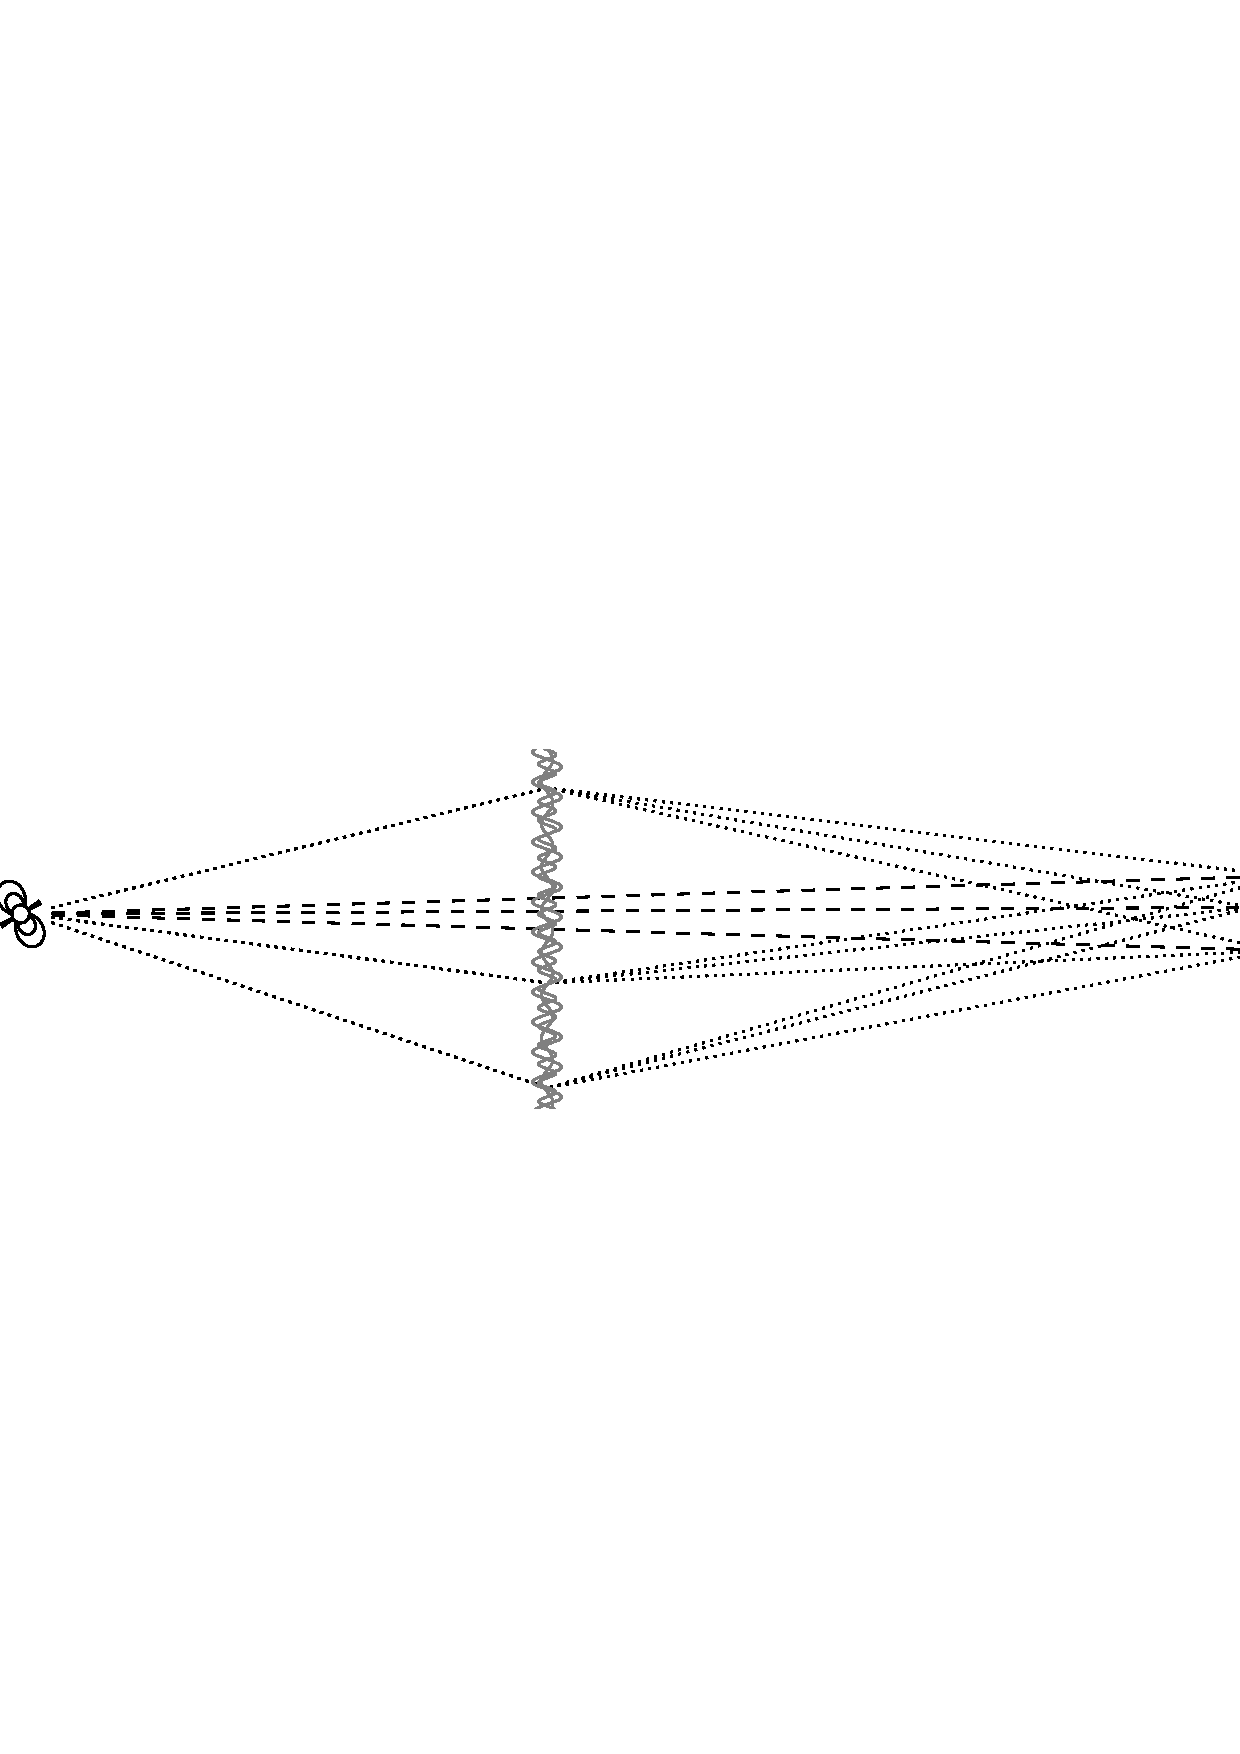
\includegraphics[width=4.5in]{Figures/scintillometry.png}
}

\end{document}
